% Compilar: cd "Diagnóstico Operacional" && pdflatex "Diagnóstico Operacional.tex"
% Figuras: ../figures/ (generadas con 01_diagnostico_operacional.ipynb)
\documentclass[11pt,a4paper]{article}
\usepackage[utf8]{inputenc}
\usepackage[T1]{fontenc}
\usepackage[spanish]{babel}
\usepackage{graphicx}
\usepackage{geometry}
\usepackage{float}
\usepackage{amsmath}
\usepackage{amssymb}
\geometry{margin=2.0cm}
\usepackage{hyperref}
\hypersetup{colorlinks=true, linkcolor=blue!50!black, urlcolor=blue!50!black}

\title{\textbf{Diagnóstico operacional}\\[0.35em]
{\large Caso técnico Rappi --- Módulo 1}\\
{\normalsize Dataset: panel 30 días $\times$ 24 h $\times$ 14 zonas (10\,080 filas)}}
\author{}
\date{\today}

\begin{document}
\maketitle

\section*{Resumen de hallazgos (máx.\ 1 página)}

\noindent\textbf{Patrones.} La \textbf{saturación} (ratio $>1.8$) representa el \textbf{5{,}09\,\%} del panel. Se concentra en franjas \textbf{12--14\,h} (picos de conteo: 14\,h, 13\,h, 12\,h) y en la tarde (\textbf{19--21\,h}). Por zona, el mayor número de observaciones en saturación aparece en \emph{San Nicolás}, \emph{Santiago}, \emph{MTY\_Guadalupe}, \emph{Carretera Nacional} y \emph{Mitras Centro}. La \textbf{precipitación} se asocia al ratio con correlación de Pearson \textbf{0{,}32} con \texttt{ratio}; en un MCO \texttt{ratio $\sim$ PRECIPITATION\_MM + HOUR + ZONE}, el coeficiente marginal es \textbf{+0{,}081} puntos de ratio por mm/h adicional (muy significativo). Condicionando el umbral de lluvia: $\mathbb{P}(\text{saturación}\mid \text{precip} > 0{,}5\,\mathrm{mm/h}) \approx 0{,}31$ frente a $\mathbb{P}(\cdot\mid \text{resto}) \approx 0{,}038$ --- un factor del orden de \textbf{$\times\,8{,}2$} en cociente de probabilidades. La sensibilidad marginal a lluvia \emph{por zona} (control por hora) es mayor en \emph{Santiago}, \emph{Carretera Nacional} y \emph{Santa Catarina}. A nivel día, la fracción de celdas saturadas llega hasta \textbf{16{,}7\,\%} en el peor día; el percentil 75 de esa fracción es \textbf{4{,}7\,\%}. La correlación Spearman global \texttt{EARNINGS}--\texttt{ratio} es débil (\textbf{0{,}08}); con precipitación $>0$ el signo se invierte respecto al agregado, coherente con que \textbf{incentivos y clima interactúan} (modelo con interacción \texttt{EARNINGS $\times$ PRECIPITATION\_MM}).

\noindent\textbf{Impacto cuantificado en la operación.} (1)~\textbf{Capacidad y pricing en ventanas críticas:} priorizar monitoreo y refuerzo de oferta en \textbf{12--14\,h} y \textbf{19--21\,h} ataca la mayor densidad observada de saturación. (2)~\textbf{Playbook de lluvia:} ante precipitación $>0{,}5$\,mm/h la probabilidad de celda saturada es \textbf{ocho veces} la de condiciones secas; conviene activar reglas de incentivos / cupos diferenciados por zona con mayor $\beta$ marginal (p.\,ej.\ Santiago y Carretera Nacional). (3)~\textbf{Eficiencia de incentivos:} la relación lineal simple incentivo--ratio es floja; revisar alineación día a día entre \textbf{earn medio} y \textbf{fracción saturada} (dispersión en P4) evita gastar en días de alto incentivo sin reducir estrés proporcionalmente. (4)~\textbf{Orden de magnitud}: el ejercicio de sensibilidad (mm/h necesarios para mover el ratio $\sim$0{,}6 puntos en el tramo saludable$\rightarrow$saturación) ordena zonas por ``fragilidad'' operativa ante lluvia (figura de sensibilidad).

\vspace{0.6em}
\noindent\rule{\linewidth}{0.4pt}

\section*{Alineación geográfica y continuidad con el Módulo 2}

\noindent El diagnóstico sobre \texttt{RAW\_DATA} debe referirse a las \textbf{mismas zonas operativas} que figuran en \texttt{ZONE\_INFO} (centroides y \texttt{DESCRIPTION}) y en \texttt{ZONE\_POLYGONS} (polígonos en WKT). En el notebook, una celda dedicada importa \texttt{validate\_excel\_zone\_consistency} desde \texttt{modulo2\_motor\_alertas/src/zones.py}: comprueba la coincidencia de nombres entre las tres hojas y cuenta cuántos WKT son parseables. Si un polígono viene \textbf{truncado} en Excel (\,$\sim$\,32\,k caracteres), no se usa para el punto de consulta; el Módulo~2 entonces toma \texttt{LATITUDE\_CENTER} y \texttt{LONGITUDE\_CENTER} de \texttt{ZONE\_INFO} (caso empaquetado: dos zonas). La misma validación se ejecuta al \textbf{recalibrar} (\texttt{export\_calibration\_from\_m1.py}) y al arrancar el motor (\texttt{run\_alert\_engine.py}), con advertencias en consola si hubiera desajustes.

\noindent La \textbf{calibración} del motor (coeficientes marginales de precipitación por zona, umbrales de alerta, sensibilidad, earnings base) se estima desde \texttt{RAW\_DATA} con la misma especificación que P3 del notebook (\texttt{ratio $\sim$ PRECIPITATION\_MM + C(HOUR)} por zona) y se escribe en \texttt{calibration.json}. El motor en vivo combina ese JSON con el \textbf{pronóstico horario} (Open-Meteo, mm/h) en coordenadas obtenidas del polígono (\texttt{representative\_point}) o, en respaldo, de los centroides anteriores. Opción \texttt{--recalibrate} en \texttt{run\_alert\_engine.py}: regenera el JSON desde el Excel antes de consultar la API.

\section*{Figuras y notas (notebook \texttt{01\_diagnostico\_operacional.ipynb})}

\noindent Las figuras se generan en el notebook (misma lógica de ratio, clasificación y modelos) y se guardan en \texttt{modulo1\_diagnostico/figures/}. A continuación se incluyen las principales para el informe.

\paragraph{P1 --- Dónde y cuándo hay saturación.}
\noindent Frecuencia por hora del día y ranking de zonas (top 14) según conteos de filas clasificadas como \texttt{saturacion}.

\begin{figure}[H]
  \centering
  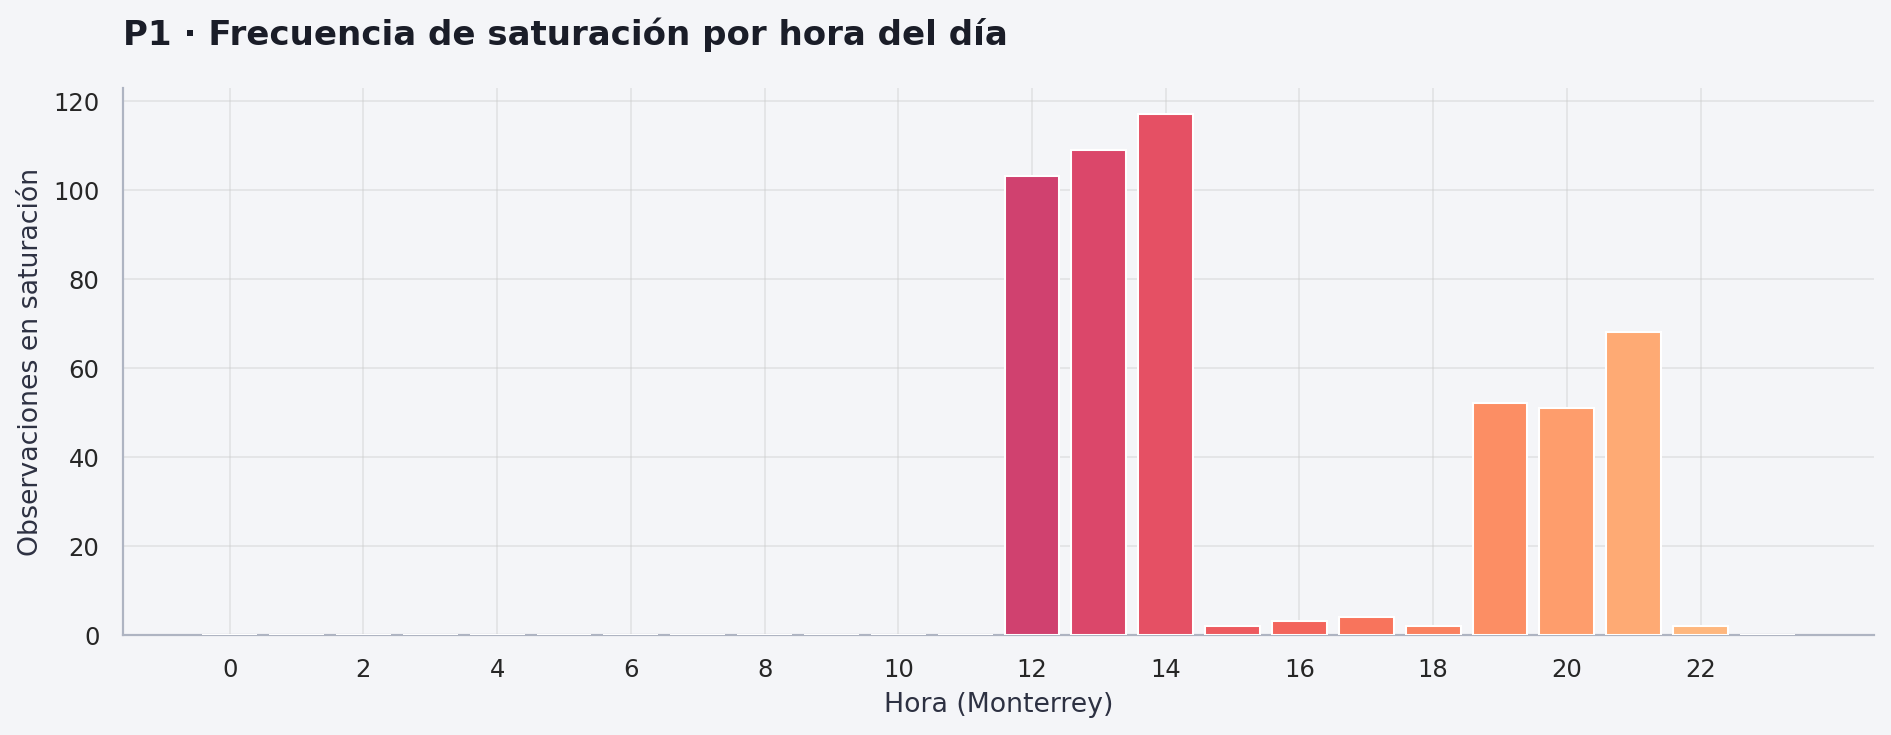
\includegraphics[width=0.48\linewidth]{../figures/p1_horas_saturacion.png}\hfill
  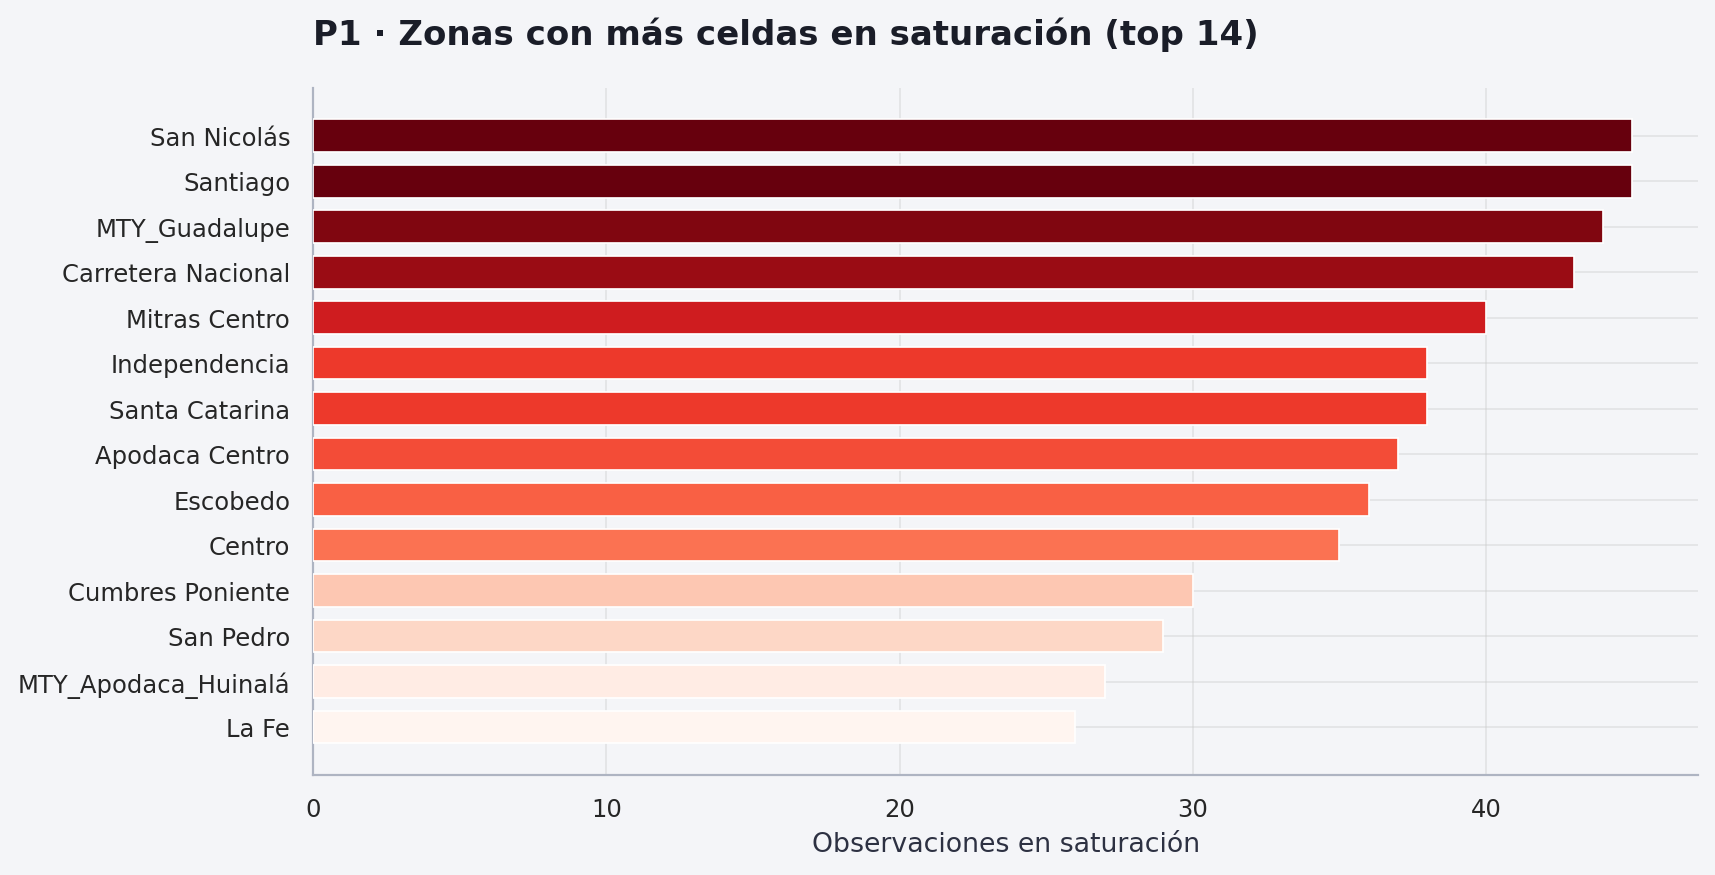
\includegraphics[width=0.48\linewidth]{../figures/p1_zonas_saturacion.png}
  \caption{P1: saturación por hora (Monterrey) y por zona.}
\end{figure}

\paragraph{P3 --- Heterogeneidad espacial (lluvia).}
\noindent Coeficiente marginal de precipitación sobre el ratio, con efectos fijos por hora dentro de cada zona.

\begin{figure}[H]
  \centering
  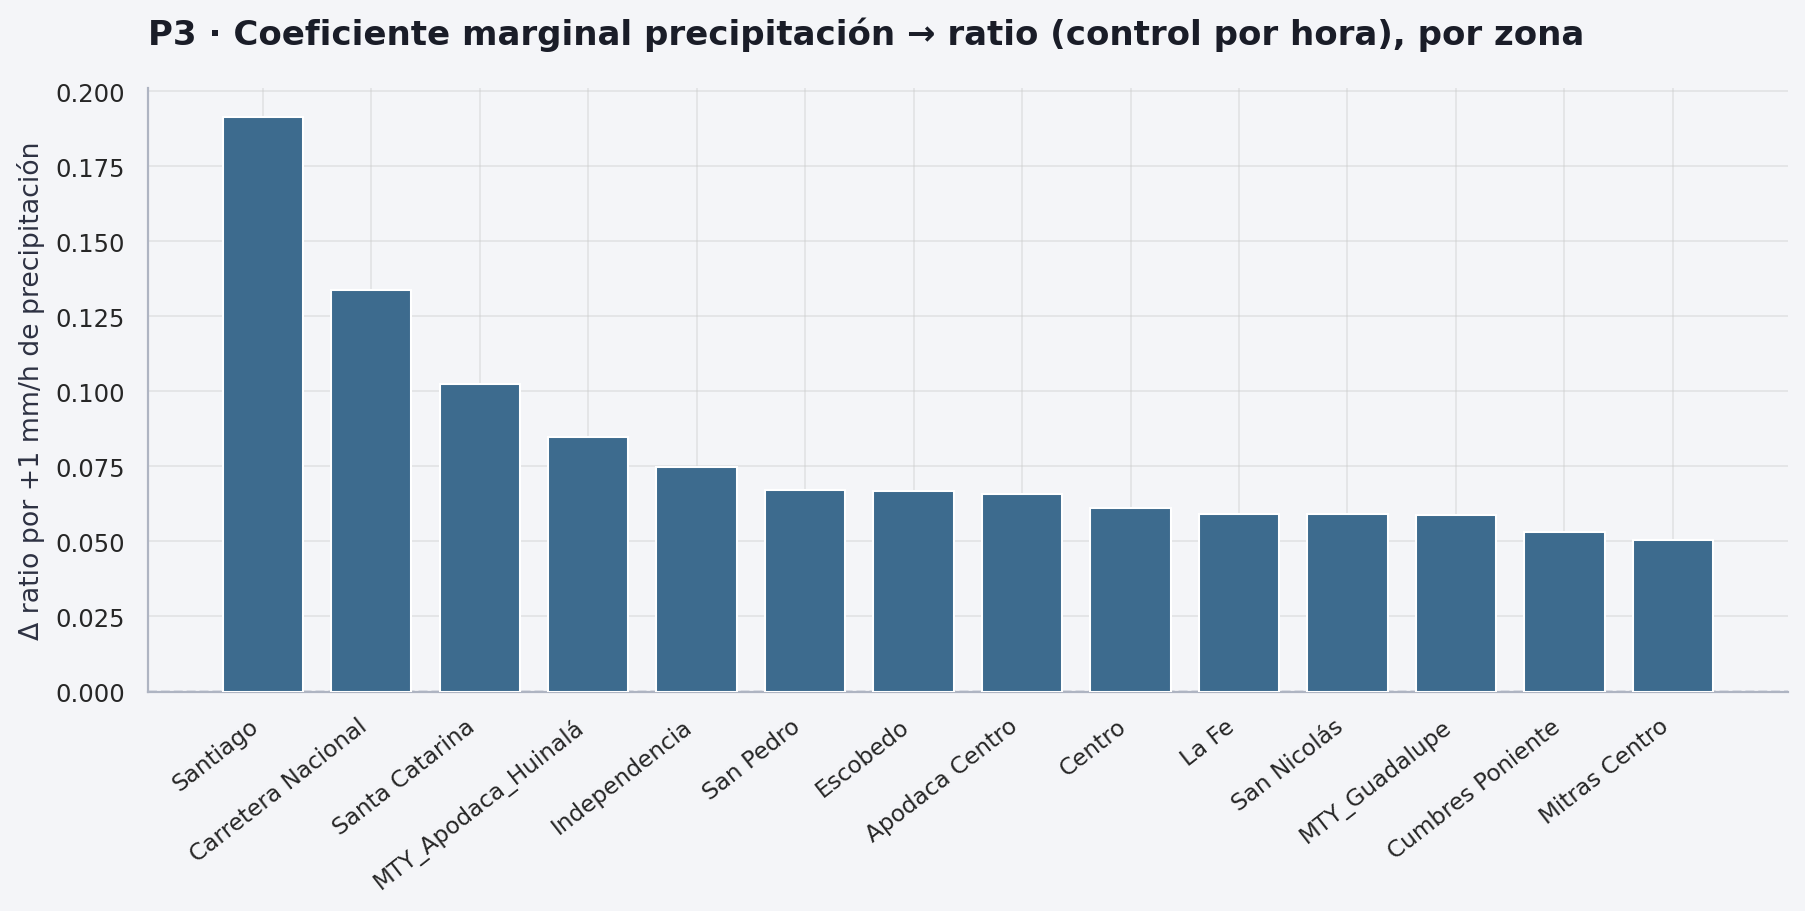
\includegraphics[width=0.82\linewidth]{../figures/p3_sensibilidad_zona.png}
  \caption{P3: sensibilidad marginal a precipitación por zona (control por hora).}
\end{figure}

\paragraph{P4 --- Earnings frente a estrés operativo.}
\noindent Cada punto es un día: incentivo medio vs.\ fracción de celdas en saturación; útil para localizar días con alto estrés y alto (o bajo) incentivo.

\begin{figure}[H]
  \centering
  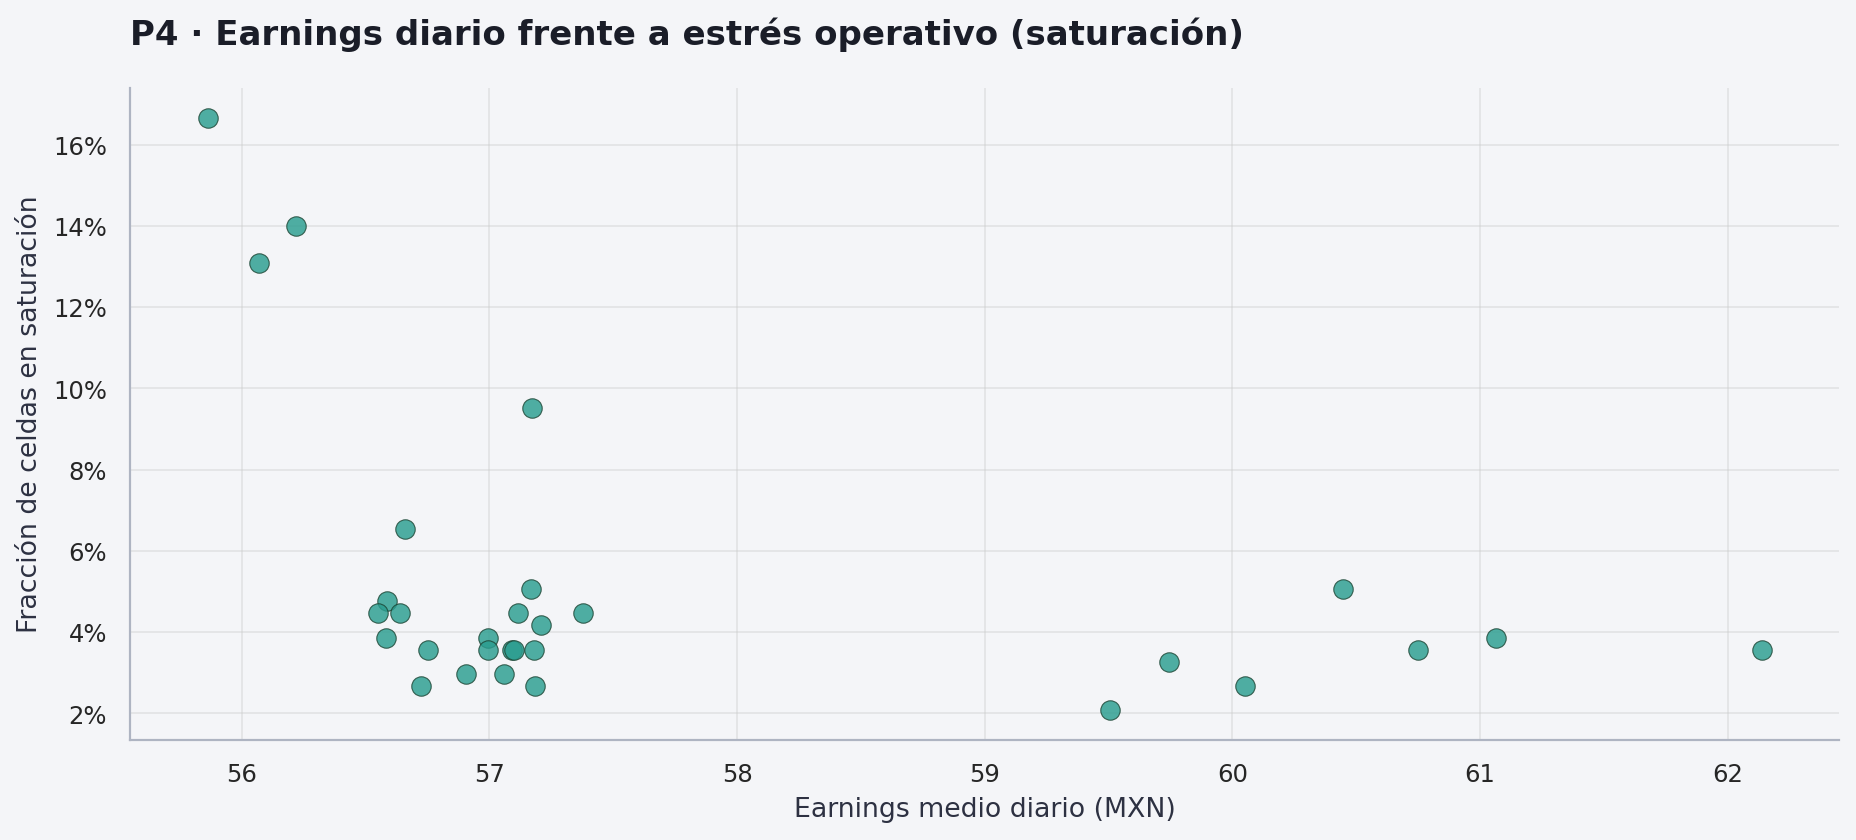
\includegraphics[width=0.82\linewidth]{../figures/p4_earnings_vs_estres.png}
  \caption{P4: dispersión diaria earn vs.\ fracción saturada.}
\end{figure}

\paragraph{Sensibilidad (orden de magnitud).}
\noindent Aproximación lineal local: mm/h adicionales asociados a un desplazamiento de ratio $\approx 0{,}6$ (tramo saludable hacia umbral de saturación), por zona.

\begin{figure}[H]
  \centering
  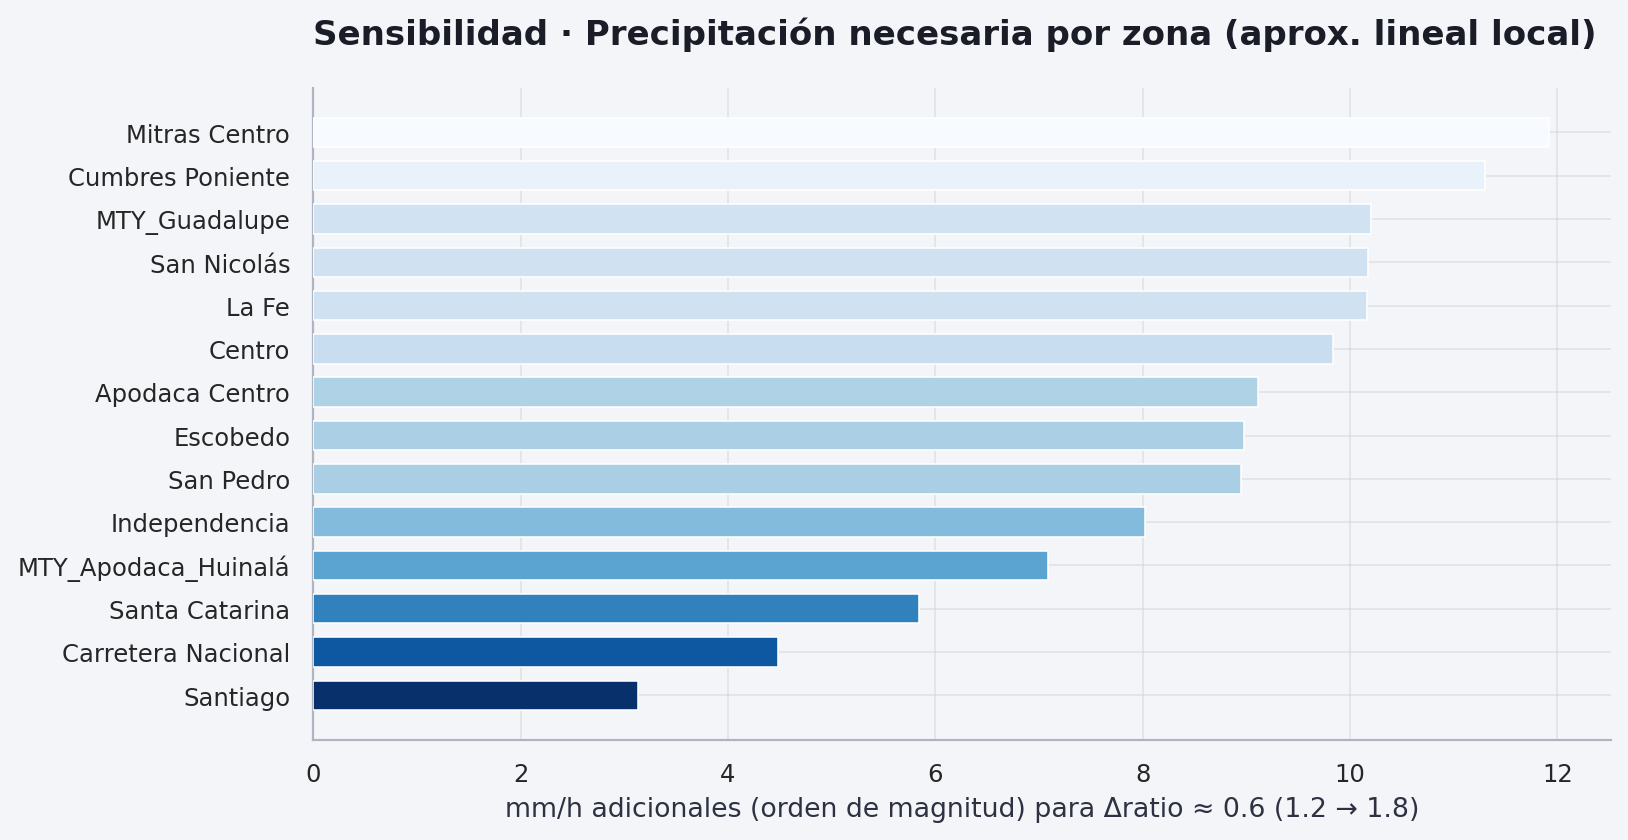
\includegraphics[width=0.82\linewidth]{../figures/p_sensitivity_mm_12_to_18.png}
  \caption{Sensibilidad: precipitación necesaria por zona (aprox.\ lineal).}
\end{figure}

\paragraph{Notas de interpretación (del notebook).}
\noindent \texttt{ratio} $=$ \texttt{ORDERS}/\texttt{CONNECTED\_RT} (si conectados $=0$, ratio vacío). Clasificación: \texttt{saturacion} ($>1{,}8$), \texttt{sobre\_oferta} ($<0{,}5$), \texttt{saludable} ($0{,}9$--$1{,}2$), \texttt{intermedio} en otro caso. P2 usa MCO con dummies de hora y zona; P3 estima por zona \texttt{ratio $\sim$ precipitación + hora}; P5 introduce interacción \texttt{EARNINGS $\times$ precipitación} para no interpretar incentivos como efecto puro sin clima.

\end{document}
